\section{Requirement Document}\label{sec:requirement-document}
\begin{figure}[H]
    \centering
    \caption[]{Requirement Document (Page 1)}
    \label{fig:requirement-document-1}
    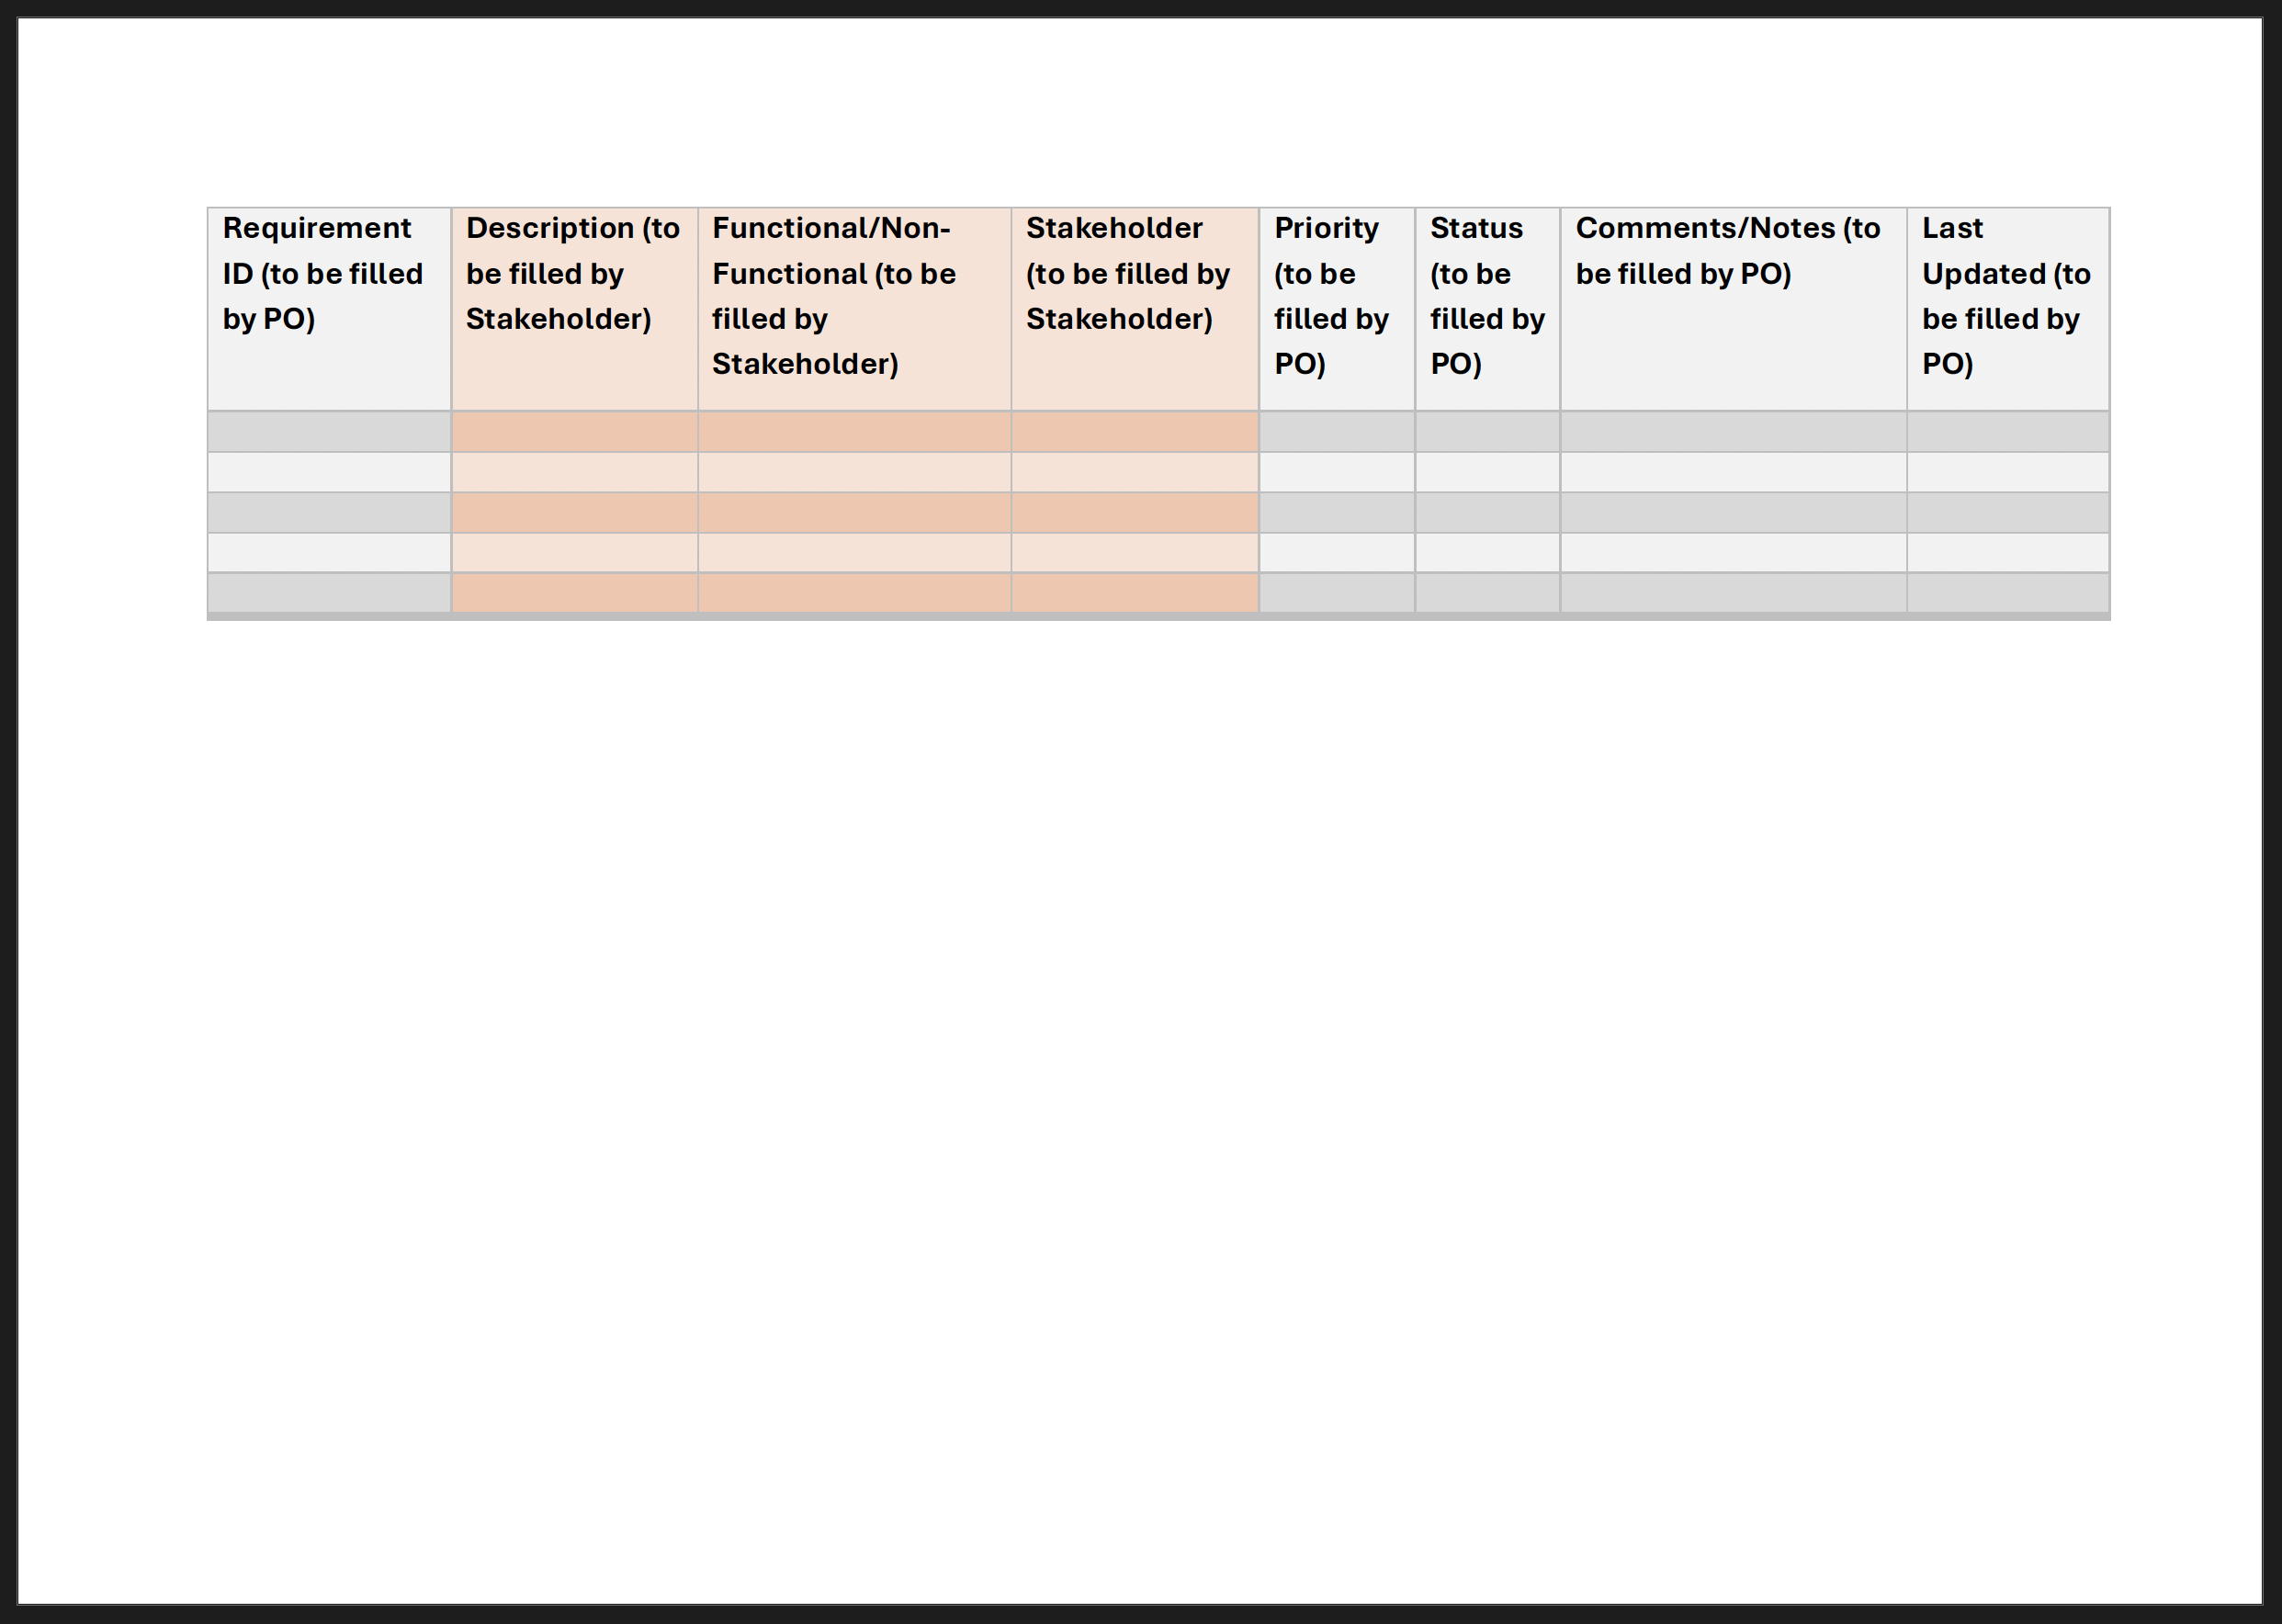
\includegraphics[width=1\textwidth]{abbildungen/RE/Word/RequirementDocument1}
\end{figure}
\begin{figure}[H]
    \centering
    \caption[]{Requirement Document (Page 2)}
    \label{fig:requirement-document-2}
    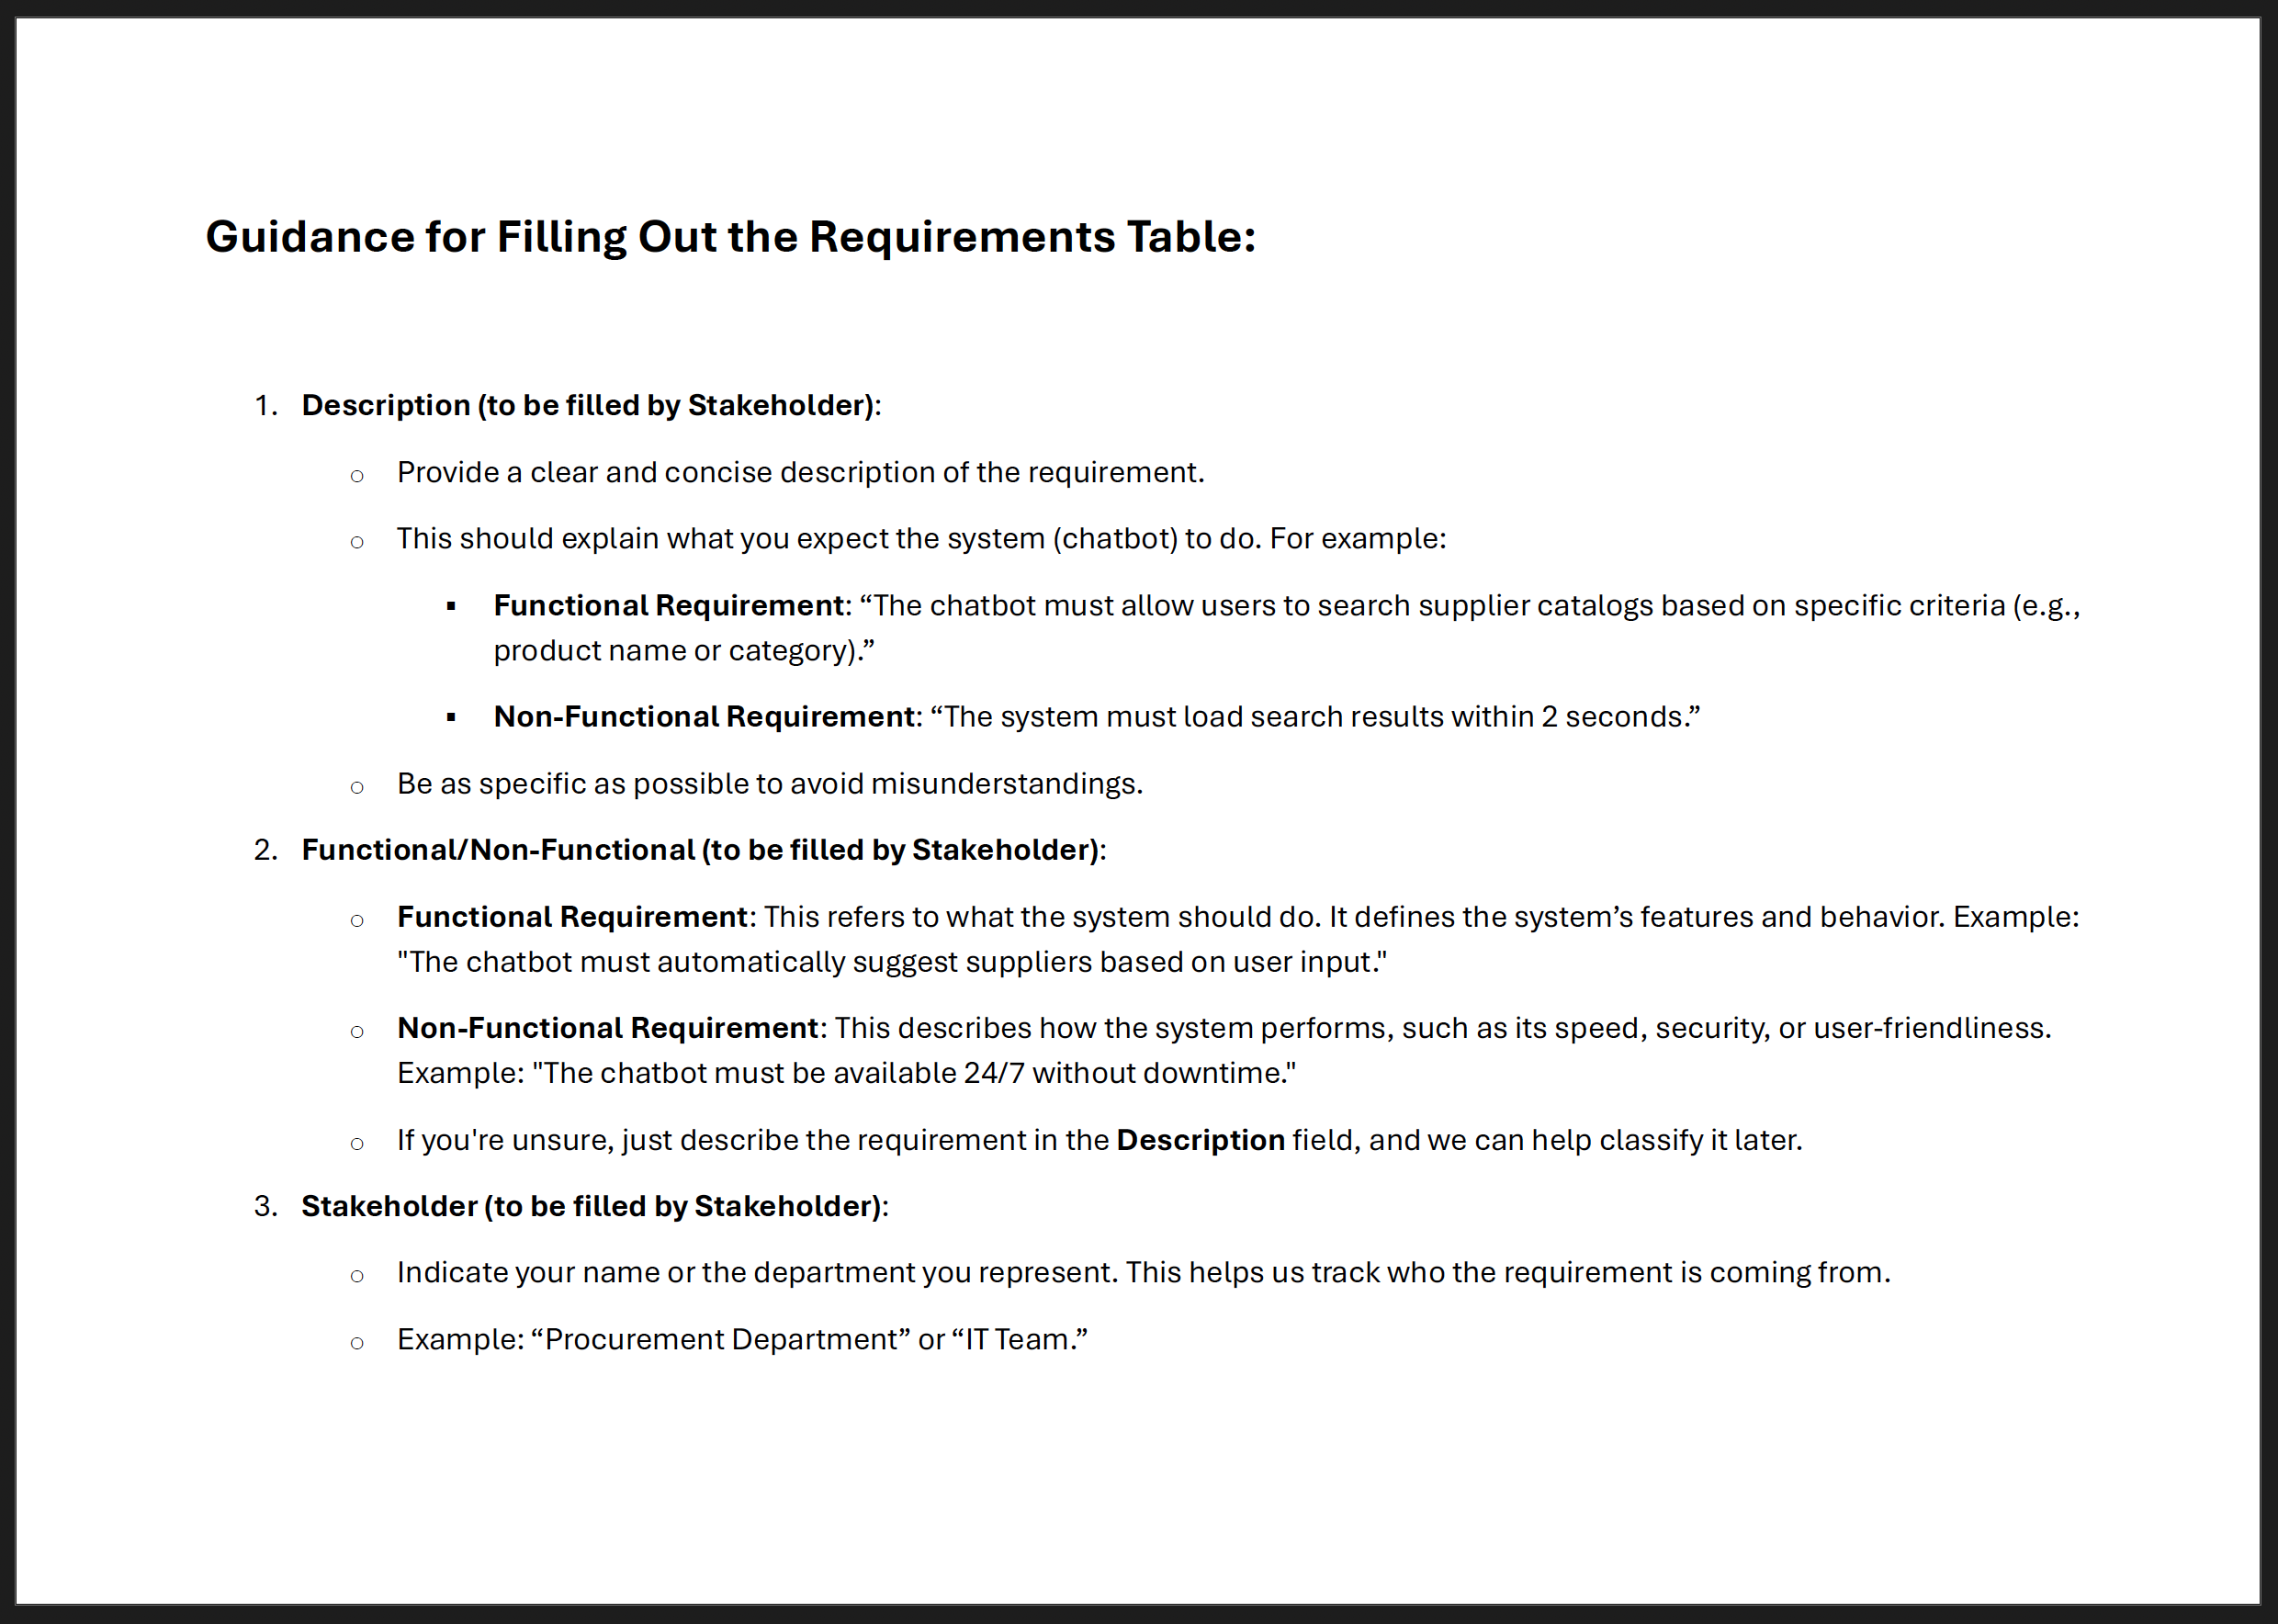
\includegraphics[width=1\textwidth]{abbildungen/RE/Word/RequirementDocument2}
\end{figure}
%TODO Anhang befüllen
\section{Requirement Elicitation}\label{sec:requirement-elicitation}
\subsection{Screen Mock-Ups in Miro}\label{subsec:screen-mock-ups-in-miro}
\subsection{Screen Prototypes in Figma}\label{subsec:screen-prototypes-in-figma}
\subsection{Filled-out Requirement Documents}\label{subsec:filled-out-requirement-documents}
\section{Prototyping}
\subsection{Frontend}\label{subsec:frontend}
\subsubsection{Example API Endpoint Definition}
% @formatter:off
\begin{lstlisting}[language=JSON, caption={Example API Endpoint Definition (\texttt{v1.json})},
  numbers=none,label={lst:api-v1-json}]
"/api/v1/cases": {
  "get": {
    "summary": "List Cases",
    "operationId": "list_cases_api_v1_cases_get",
    "parameters": [
      {
        "name": "user_id",
        "in": "query",
        "required": false,
        "schema": {
          "anyOf": [
            { "type": "string" },
            { "type": "null" }
          ],
          "title": "User Id"
        }
      },
      {
        "name": "limit",
        "in": "query",
        "required": false,
        "schema": {
          "anyOf": [
            { "type": "integer" },
            { "type": "null" }
          ],
          "default": 10,
          "title": "Limit"
        }
      }
    ]
  },
  "post": {
    "summary": "Create Case",
    "operationId": "create_case_api_v1_cases_post",
    "requestBody": {
      "required": true,
      "content": {
        "application/json": {
          "schema": {
            "$ref": "#/components/schemas/CreateCaseRequest"
          }
        }
      }
    }
  }
}
\end{lstlisting}
% @formatter:on
